\documentclass[12pt, a4paper]{article}
\usepackage{ctex}
\usepackage{graphicx}
\usepackage{amsthm}
\usepackage{amsmath}
\usepackage{amsfonts}
\usepackage{amssymb}
\usepackage[margin = 1in]{geometry}
\usepackage{enumerate}
\usepackage{multicol}
\usepackage{fancyhdr}
\usepackage{ifthen}
\usepackage{syntonly}
\usepackage{color}
\usepackage{makecell}
\usepackage{eufrak}
\usepackage{comment}
\usepackage[bitstream-charter]{mathdesign}
\usepackage[T1]{fontenc}
\usepackage[colorlinks, CJKbookmarks=true, linkcolor=black, anchorcolor=blue, citecolor=blue]{hyperref}
\pagestyle{fancy}

%\fancyhf{} % sets both header and footer to nothing
\lhead{}
\chead{}
\rhead{}
\renewcommand{\headrulewidth}{0pt}

\renewcommand\contentsname{Contents}
\renewcommand\refname{References}
\renewcommand\figurename{Fig.}
\newcommand{\upcite}[1]{\textsuperscript{\textsuperscript{\cite{#1}}}}

\newcounter{footnotesintable}

\begin{document}


\title{Project Report of RISC-V CPU\\\begin{large}(Course Project of Computer Architecture)\end{large}}
\author{Weixin Deng {\kaishu{(邓伟信})}\\ACM Class, Shanghai Jiao Tong University}
\date{}

\maketitle

\section{Introduction}

This project is a RISC-V CPU with a five-stage pipeline, implemented in Verilog HDL. The GitHub repository of my CPU project is: \url{https://github.com/dengwxn/RISC-V-CPU}.

\section{Implementation}


\begin{comment}
\begin{table}[!hbp]
	\centering
	\setcounter{footnotesintable}{0}
	\begin{tabular}{|l|l|}
		\hline
		\multicolumn{1}{|c|}{Feature} & \multicolumn{1}{c|}{RISC-V CPU} \\ \hline
		ISA & RV32I\addtocounter{footnote}{1}\addtocounter{footnotesintable}{1}\footnotemark[\thefootnote] \\ \hline
		Pipelining & 5 stages \\ \hline 
		Data forwarding & complete forwarding path \\ \hline
	\end{tabular}
\end{table}
\addtocounter{footnote}{-\thefootnotesintable}
\addtocounter{footnote}{1}\footnotetext[\thefootnote]{except \textit{FENCE*, ECALL, EBREAK, CSRR*}.}
\end{comment}

\begin{figure}[!ht]\centering
	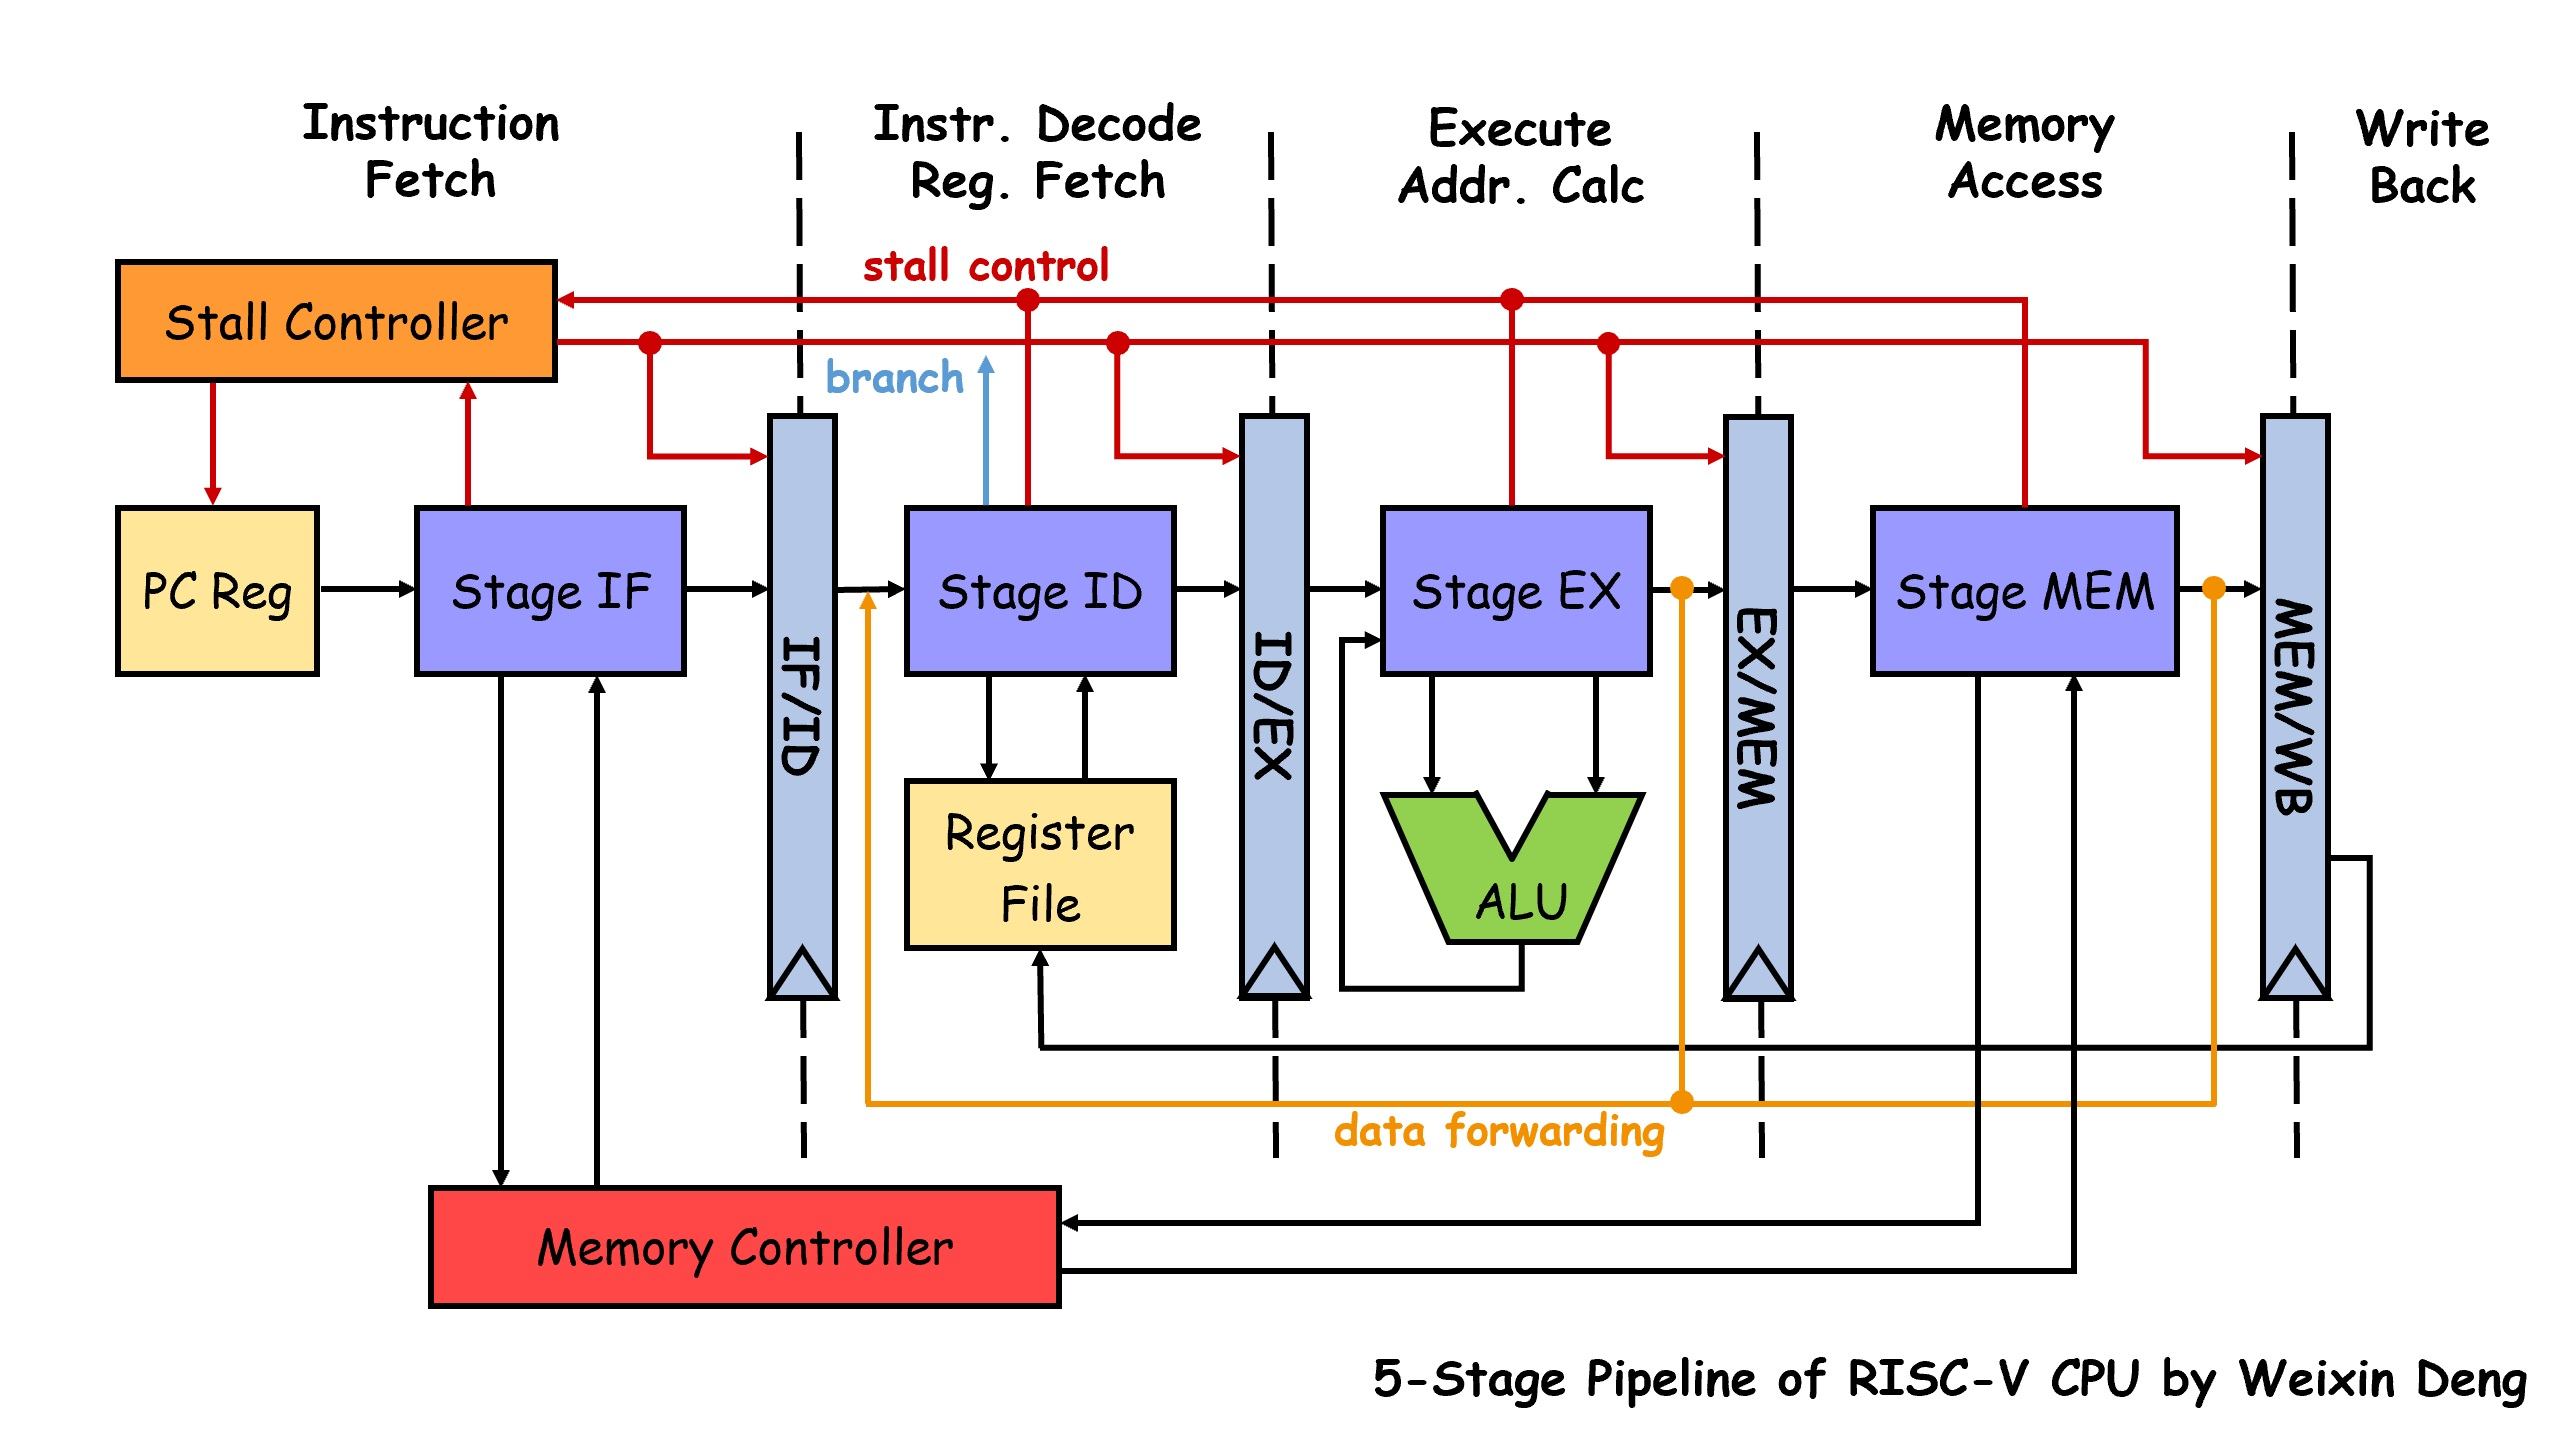
\includegraphics[scale=0.23]{graph.jpg}
	\caption{Overview of CPU Design}
\end{figure}

My CPU has a RV32I\footnote{except \textit{FENCE*, ECALL, EBREAK, CSRR*}.} ISA, and has a standard 5-stage pipeline with data forwarding. It always predicts branches are not taken and does not have an instruction cache or a data cache. All test programs run correctly on FPGA.

\begin{itemize}
	\item 
	Data produced by EX and MEM is passed to ID, which can avoid most of RAW data hazards. The pipeline still needs to stall when the producer is a \textit{load} instruction.
	\item 
	For a \textit{branch} instruction, the branch address is given in ID. 
	\item 
	In this project, the memory module given can read or write only one-byte data per time, so it takes multiple cycles to finish IF and MEM and the pipeline need to stall as well. Then it's necessary to implement an instruction cache and a data cache for better performance but I did not succeed before the deadline.
	\item 
	Because IF and MEM might need to access memory at the same time if having cache misses, I implement a memory controller which receives requests, sends back data and runs like a deterministic finite automaton.   
\end{itemize}

\section{Discussions}

\paragraph{Debug} 
I think Verilog HDL is different from other languages like C++ when debugging, though they are similar in syntaxes. One practical way to debug is checking the waveform configuration (WCFG), which is in some sense similar to debug C++ using GDB. Sometimes we'd like to know in \textit{if-else} and \textit{case} blocks which branch my program jumps into. And we can set up some regs which change their values inside different branches and add them in the WCFG (proposed by Zhaoyu Li).

\paragraph{Verilog and FPGA}
At the beginning, I was not sure about the distinctions between wire and reg, until I found an document.\upcite{wire and reg} Besides, some potential faults might be invisible in simulations. One common mistake is generating latches, which probably brings unexpected results. And it is thoroughly discussed in this document.\upcite{always} I strongly recommend to read these two documents before starting the CPU project, which is helpful to get the CPU running correctly on FPGA.

\paragraph{Pipeline}
It took me a while to understand functions of combinational logic and sequential logic. In a pipeline, sequential logic drives an instruction to the next stage and latency of combinational logic determines the clock rate and therefore the performance. Technically, my CPU does not have a real pipeline considering that I did not implement an instruction cache. Thus, when I finish fetching the next instruction, all stages of the last instruction are probably finished (unless the last instruction is \textit{load} or \textit{store}). Namely, the correctness of my CPU pipeline remains to be verified.

\section{Acknowledgements}

I am grateful to Linqi Chen {(\kaishu{陈林淇})}, Qidong Su {(\kaishu{苏起东})} and Zhaoyu Li {(\kaishu{李照宇})} who have shared their experience with me and provided much guidance. Besides, I would like to express my gratitude to TA Yunfeng Lin {(\kaishu{林耘丰})} and TA Yuxi Liu {(\kaishu{刘予希})} for their great work on the project and the course. And I also thank many other classmates for their direct and indirect help to me. 

\section{Appendix}

\begin{thebibliography}{9}
  \bibitem{lsl}
  	雷思磊.
  	\emph{自己动手写CPU},
  	电子工业出版社, 2014.
  \bibitem{CSAP} 
	Randal E. Bryant and David R. O'Hallaron.
	\emph{Computer Systems: A Programmer's Perspective, (CS:APP)},
	Third Edition, 2015.
  \bibitem{zhoufan}
  	Zhou Fan's RISC-V CPU project.
	\url{https://github.com/Evensgn/RISC-V-CPU}.
  \bibitem{wire and reg}
  	Chris Fletcher.
	  \emph{Verilog: wire VS. reg}.
	  \\\url{https://inst.eecs.berkeley.edu/~cs150/Documents/Nets.pdf}.
  \bibitem{always}
  	Chris Fletcher.
	  \emph{Verilog: always @ Blocks}.
	  \\\url{http://inst.eecs.berkeley.edu/~cs150/fa08/Documents/Always.pdf}.
  
\end{thebibliography}

\end{document}